\documentclass[../../relatorio.tex]{subfiles}

\begin{document}

\subsection{Produto Interno Bruto - PIB}

\begin{figure}[ht]
  \begin{minipage}{0.30\textheight}
    \centering
      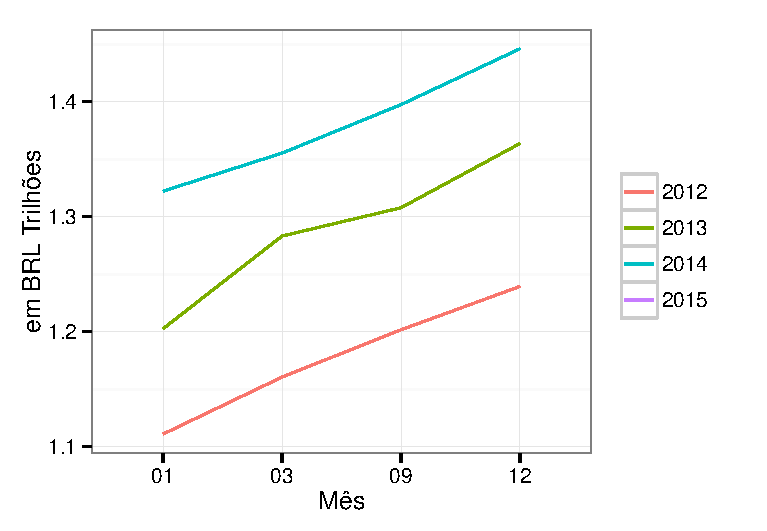
\includegraphics{PIB.pdf}
  \end{minipage}
\end{figure}


O produto interno bruto (PIB) representa a soma (em valores monetários) de todos os bens e serviços finais produzidos numa determinada região (quer sejam países, estados ou cidades), durante um período determinado (mês, trimestre, ano, etc). O PIB é um dos indicadores mais utilizados na macroeconomia com o objetivo de mensurar a atividade econômica de uma região.

Na contagem do PIB, considera-se apenas bens e serviços finais, excluindo da conta todos os bens de consumo de intermediário. Isso é feito com o intuito de evitar o problema da dupla contagem, quando valores gerados na cadeia de produção aparecem contados duas vezes na soma do PIB. \footnote{http://pt.wikipedia.org/wiki/Produto\_ interno\_ bruto}


\pagebreak

\end{document}
